\documentclass{article}
\usepackage[a4paper, total={6in, 10in}]{geometry}
\usepackage[utf8]{vietnam}
\usepackage{cite}
\usepackage{float}
\usepackage{graphicx}
\usepackage{lmodern}
\usepackage{minted}
\usepackage{hyperref}

\begin{document}
\title{
	\LARGE{
		\textbf{
			Xây dựng mô hình Machine Learning \\ dự báo cháy rừng ở các tỉnh Tây Nguyên \\ dựa vào dữ liệu lịch sử thời tiết.
		}
	}
}

\author{
	Nguyễn Đại Kỳ\\
	19521731\\
	\and
	Văn Viết Hiếu Anh\\
	19521225
	\and
	Lê Văn Phước\\
}

\date{\today} % Date for the report
\maketitle % Insert the title, author and date
\begin{center}
	\begin{tabular}{l l}
		Môn học:              & CS114 - Máy học       \\
		Giảng viên hướng dẫn: & Lê Đình Duy           \\
		                      & Phạm Nguyễn Trường An \\
	\end{tabular}
\end{center}

\tableofcontents

\pagebreak

%----------------------------------------------------------------------------------------
%	SECTION 1
%----------------------------------------------------------------------------------------

\section{Tổng quan}
\qquad Bài viết là về quá trình thực nghiệm nghiên cứu các model Machine Learning với mục đích chọn ra mô hình tối ưu để dự đoán mức độ cháy rừng dựa vào dữ liệu thời tiết trong lịch sử của từng địa phương. Với mục đích hổ trợ trong việc dự đoán để phục vụ trong công tác phòng chống cháy rừng ở nước ta. Vì bài viết là ghi chép của quá trình thực nghiệm nên sẽ có nhiều phương pháp được đưa ra sử dụng.

\subsection{Mô tả bài toán}
\qquad Ở nước ta có 3 thảm họa lớn nhất, gây thiệt hại lớn hàng năm về cả người và của. Cùng với lũ lụt và hạn hán, cháy rừng là một thảm họa gây thiệt hại không chỉ về kinh tế mà còn cả con người và hệ sinh thái. Theo thống kê của Cục Kiểm lâm từ năm 1992 đến 2006, trung bình mỗi năm xảy ra 1254 vụ cháy rừng gây thiệt hại khoảng 6646 ha rừng, trong đó có 2854 ha là rừng tự nhiên và 3791 ha là rừng trồng. Bên cạnh việc nâng cao năng lực phòng cháy chữa cháy rừng (PCCCR) cho lực lượng kiểm lâm như đầu tư trang thiết bị, cơ sở vật chất, xây dựng cơ chế điều hành phối hợp và tuyên truyền nâng cao nhận thức trách nhiệm của chủ rừng và người dân, công tác cảnh báo nguy cơ cháy rừng cũng như tổ chức phát hiện sớm và thông báo kịp thời điểm cháy rừng là rất cần thiết.

Từ đầu năm 2007, Cục Kiểm lâm (Bộ Nông nghiệp và Phát triển Nông thôn) đã lắp đặt và vận hành trạm thu ảnh viễn thám MODIS tại Hà Nội với mục đích chính là phát hiện sớm các điểm cháy rừng (hotspots) trên toàn lãnh thổ Việt Nam. Hệ thống trạm thu của TeraScan đã tự động thu nhận, xử lý và sao lưu dữ liệu ảnh MODIS hàng ngày từ 2 vệ tinh TERRA và AQUA với mô-đun Vulcan tự động xử lý và tạo ra dữ liệu các điểm cháy sử dụng thuật toán ATBD-MOD14\cite{website:atbd-mod14}.

Hệ thống này cung cấp dữ liệu về điểm cháy ghi nhận được từ vệ tinh và lưu lại thời gian và tọa độ cháy. Từ khi bắt đầu lắp đặt đến nay hệ thống dữ liệu cháy của cục kiểm lâm được ghi lại được gần 1 triệu điểm cháy. Nhờ lượng dữ liệu này việc xây dựng một hệ thống tự động phân tích mức độ cháy rừng dựa vào các đặc trưng cơ bản của dữ liệu khí tượng thủy văn là hoàn toàn có cơ sở và khả quan.

Input của bài toán là dữ liệu lịch sử thời tiết trong vòng 1 tháng trở lại và từ đó để model đánh giá địa phương đó vào ngày mai có mức độ cháy được đánh giá ở thang nào.

Chưa làm xong đâu, làm phụ đi

\subsection{Mô tả dữ liệu}

Nguồn dữ liệu của nhóm đến từ các website gồm 3 website chính:

\begin{itemize}
	\item firewatchvn.kiemlam.org.vn: là Hệ thống theo dõi cháy rừng trực tuyến thuộc Cục Kiểm Lâm - Tổng cục Lâm Nghiệp
	\item weather.com: là website của The Weather Channel (TWC) - IBM\cite{website:wiki_twc}
	\item worldweatheronline.com
\end{itemize}

Trong 3 nguồn dữ liệu thì chỉ có worldweatheronline.com sử dụng SSR(Server-side render) còn 2 nguồn còn lại đều sử dụng Ajax để truyền dữ liệu qua lại giữa server.

\subsubsection{Weather Data}
\qquad\emph{Việc tìm các nguồn dữ liệu khác về thời tiết ngoài 2 nguồn trên đã được thực hiện song các nguồn này đều có những điểm thiếu rất quan trọng ví dụ như API của website chỉ cung cấp trong 1 năm trở lại hay các website này không cung cấp đủ nhiều địa phương mà chỉ cung cấp dữ liệu ở những thành phố cụ thể.}

Có thể nói việc lấy dữ liệu thời tiết là công đoạn gây ra nhiều khó khăn nhất. Đa phần dữ liệu lịch sử thời tiết là rất lớn và các công ty hay tập đoàn công nghệ đều dùng để bán chứ không public trên website của họ. Ngay cả trên giao diện chính của weather.com của IBM cũng chỉ hiển thị dữ liệu thời tiết trong 2 năm trở lại (tức là 2021 và 2020).

Tuy nhiên vì sử dụng Ajax nên sau khi phân tích và ghi lại các request mà website gửi đi cũng như các response nhận về, việc có thể tìm được các cổng API và phương thức giao tiếp với server, từ đó dùng vào việc khai thác dữ liệu tự động trong nhiều năm trước nữa là hoàn toàn có hy vọng.

Về việc tìm nguồn dữ liệu tương tự đã được khai thác trước, nhóm đã từng thử tìm kiếm nhưng để đạt được yêu cầu chi tiết đến từng địa phương với thời gian kéo dài thì không tìm được dữ liệu nào đạt yêu cầu. Ngay cả khi join vào Slack của \href{https://callforcode.org/}{Call For Code} năm nay để xin hỗ trợ vì đề tài này có liên quan đến cuộc thi thì phía ban tổ chức cuộc thi cũng trả lời rằng dữ liệu này không cung cấp cho thí sinh. Ngoài ra nhóm cũng đã thử gửi mail cho Trung tâm Dự báo khí tượng thuỷ văn quốc gia nhưng cũng không nhận được phản hồi. Hiển nhiên, việc tự đi thu thập dữ liệu là tất yếu.

\subsubsection{Fire Data}
\qquad firewatchvn.kiemlam.org.vn là website tạo ra ý tưởng cho nhóm. Website này cung cấp giao diện tra cứu dữ liệu về các điểm cháy vào từng thời gian cụ thể. Tuy nhiên điểm yếu của website này là xây dựng quá nhiều tính năng và sử dụng Ajax nên dùng những công cụ như Beautiful Soup thì không thể thu thập còn nếu dùng những công cụ như Selenium hay Puppeteer thì tốc độ quá chậm (dữ liệu này kéo dài từ 1/1/2008 đến 5/12/2020 nếu tra cứu từng ngày trên 700 quận, huyện, thành phố thuộc tỉnh,... thì sẽ mất rất nhiều thời gian). Điều này bắt buộc nhóm phải phân tích API mà website đã lấy dữ liệu điểm cháy để tăng tốc độ lấy dữ liệu. Bởi vì những thông tin như bản đồ của địa điểm lấy dữ liệu là không cần thiết, ta hoàn toàn có thể lấy bản đồ địa hình của cả trái đất chỉ cần dùng tọa độ. Việc lấy những thông tin nặng như bản đồ cần thời gian tải rất lâu nên việc tìm ra API mà website sử dụng cũng là cần thiết.


%----------------------------------------------------------------------------------------
%	SECTION 2
%----------------------------------------------------------------------------------------

\section{Các nghiên cứu trước}
% Chương này trình bày các kết quả nghiên cứu đã có của tiền nhân liên quan đến bài toán mà nhóm chọn. Những nghiên cứu trước làm trên các bộ dữ liệu nào, dùng phương pháp nào và performance đạt được bao nhiêu
% Nếu có khả năng thì phân tích thêm kết quả của họ như vậy là tốt chưa, có còn chỗ gì để cải thiện không. Nếu không nhận xét dược thì thôi.
\subsection{Predicting Australia wildfires with weather data a Call For Code spot challenge of IBM}
Mục đích của cuộc thi này là dự đoán kích thước của khu vực cháy tính bằng km2 theo khu vực ở Úc cho mỗi ngày trong tháng 2 năm 2021 bằng cách sử dụng dữ liệu có sẳn cho đến ngày 29 tháng 1.
Bài toán chuỗi thời gian dựa trên dữ liệu hàng ngày do Pairs Geoscope cung cấp.
Dữ liệu được cung cấp bao gồm:
\begin{itemize}
	\item Những trận cháy rừng trong lịch sử
	\item Thời tiết lịch sử
	\item Các dự báo thời tiết lịch sử
	\item Chỉ số thảm thực vật lịch sử
	\item Các loại đất của các địa điểm xảy ra cháy rừng.
\end{itemize}
Trong đó dữ liệu thời tiết lịch sử bao gồm các trường như \textbf{vùng}, \textbf{thời gian}, \textbf{lượng mưa (mm/ngày)}, \textbf{Độ ẩm tương đối (\%)}, \textbf{Hàm lượng nước trong đất ($m^3$/$m^3$)}, \textbf{bức xạ mặt trời (MJ/ngày)}, \textbf{nhiệt độ (C)}, \textbf{tốc độ gió (m/s)}. Đây là dữ liệu chính áp dụng vào bài toán của nhóm. Tuy nhiên vì khó khăn trong việc tìm kiếm dữ liệu nên nhóm chỉ đáp 4/6 tiêu chí mà các chuyên gia đã đưa ra đó là lượng mưa, độ ẩm, nhiệt độ, tốc độ gió.

Từ những nghiên cứu các chuyên gia đưa ra các biến ảnh hưởng đến cháy rừng như:
\begin{itemize}
	\item Lãnh thổ:
	      \begin{itemize}
		      \item Khu vực: Số lượng và cường độ đám cháy khác nhau ở các khu vực khác nhau. Các sự kiện ở các khu vực lân cận có thê ảnh hưởng đến cháy rừng trong một lãnh thổ nhất định. Thành phần tự phục hồi( sự diện diện của cháy rừng trong những ngày trước đó).
		      \item Tính theo mùa: Cháy rừng đặc biệt dữ dội trong “Mùa cháy rừng” kéo dài từ tháng 10 đến tháng 12. Quan sát này sẽ ảnh hưởng đến cách thức phân chia tập dữ liệu huấn luận và kiểm tra.
	      \end{itemize}
	\item Điều kiện đất và khí quyển:
	      \begin{itemize}
		      \item Thời tiết và đất đai: Thời tiết và Hạn hán có liên quan chặt chẽ đến hỏa hoạn. So sánh giữa lịch sử và dự báo thời tiết trong lịch sử.
		      \item Thảm thực vật: Có mối tương quan thuận giữa sự thay đổi chỉ số thảm thực vật và cường độ cháy.
		      \item Sử dụng đất: Việc sử dụng đất có thể liên quan đến việc dự đoán sự kéo dài của cháy rừng. Tuy nhiên, dữ liệu này chỉ có sẳn dưới dạng một hàng – cho mọi khu vực, do đó nó không được đưa vào mô hình.
	      \end{itemize}
\end{itemize}
Theo báo các tổng kết cuộc thi thì mô hình được sử dụng là Convolutional Neural Network (Windowing Dataset, Conv1D Layers,…) cho ra kết quả RMSE: 19.96, MAE: 6.94, TOT: 9.54
Qua nghiên cứu của cuộc thi này nhóm rút ra được các biến ảnh hưởng đến cháy rừng, cách khai thác lấy dữ liệu từ thực tế, mô hình đào tạo phù hợp với bài toán.
\subsection{AI and Climate data for predicting fire frequency in California}
Mục đích của nghiên cứu này là dự đoán tần suất xảy ra cháy rừng có thể giúp lập kế hoạch khẩn cấp và chủ động quản lý rủ ro thiên tai.
Dữ liệu về đám cháy được thu từ Kaggle(\url{https://www.kaggle.com/rtatman/188-million-us-wildfires}), bao gồm khoảng 1,9 triệu vụ cháy rừng ở Mỹ được tham chiếu trong giai đoạn 1992-2015. Ngoài ra, dữ liệu khí hậu từ Copernicus ERA5 được tải xuống và sử dụng cho bài toán này.

Bài nghiên cứu này cũng đưa ra kết luận về việc cháy rừng thường xảy ra hàng tháng hoặc theo mùa. Ở đây, các chuyên gia đưa ra các trường dữ liệu thời tiết được lấy là \textbf{total\_precipitation}, \textbf{2m\_temperature}, \textbf{2m\_dewpoint\_temperature}, \textbf{10m\_wind\_speed}, \textbf{volumetric\_soil\_water}, \textbf{potential\_evaporation}.

Qua nghiên cứu, bài báo đã tính toán hệ số tương quan giữa tuần suất các đám cháy và điều kiện khi hậu trung bình. Phân tích chỉ ra mối tương quan cao đáng kể giữa nhiệt độ mùa hè và PET với số lượng các sự kiện cháy ở CA.

Mô hình dữ đoán trong nghiên cứu này khá đơn giản và nó chỉ sử dụng 6 biến khi hậu được tính trung bình trên toàn California để dự đoán tần suất cá đám cháy trong tiểu bang. Sử dụng tensorflow và scikit-learning để phát triển mạng nơ-ron nhân tạo dựa trên hồi quy.

Từ đánh giá mô hình của bài nghiên cứu cho ra sai số tuyệt đối trung bình tương đối hàng năm (RMAE) khoảng 10\%.

Qua nghiên cứu trên, nhóm cũng rút ra được các biến dữ liệu cần thiết và tác động lớn đến cháy rừng, các phương pháp xử lý số liệu và mô hình được đề xuất sử dụng cho loại bài toán này là ANN.
%----------------------------------------------------------------------------------------
%	SECTION 3
%----------------------------------------------------------------------------------------
\section{Xây dựng bộ dữ liệu}
\qquad Chương này mô tả quá trình thu thập dữ liệu. Nếu dữ liệu crawling tự động thì mô tả cách viết crawler, các khó khăn gặp phải và các số liệu liên quan. Nếu dữ liệu thu thập thủ công thì mô tả các tiêu chí đặt ra để thống nhất trong nhóm khi thu thập. Làm sao để đảm bảo bộ dữ liệu thu thập thủ công có thể khớp gần giống với ngữ cảnh ứng dụng của bài toán.

Sau đó mô tả các thông số chi tiết của bộ dữ liệu, kèm theo ví dụ minh họa rõ ràng. Bài toán đặt ra các trường hợp dữ liệu nào là khó xử lý, có bao nhiêu mẫu dữ liệu thuộc trường hợp đó, chụp vài mẫu dữ liệu khó đó vào báo cáo để minh họa.

\subsection{Quá trình thu thập dữ liệu}

Tất cả dữ liệu của nhóm đều bắt đầu bằng 1 quy trình chung để kiểm tra xem nguồn dữ liệu có đáp ứng các yêu cầu hay không.

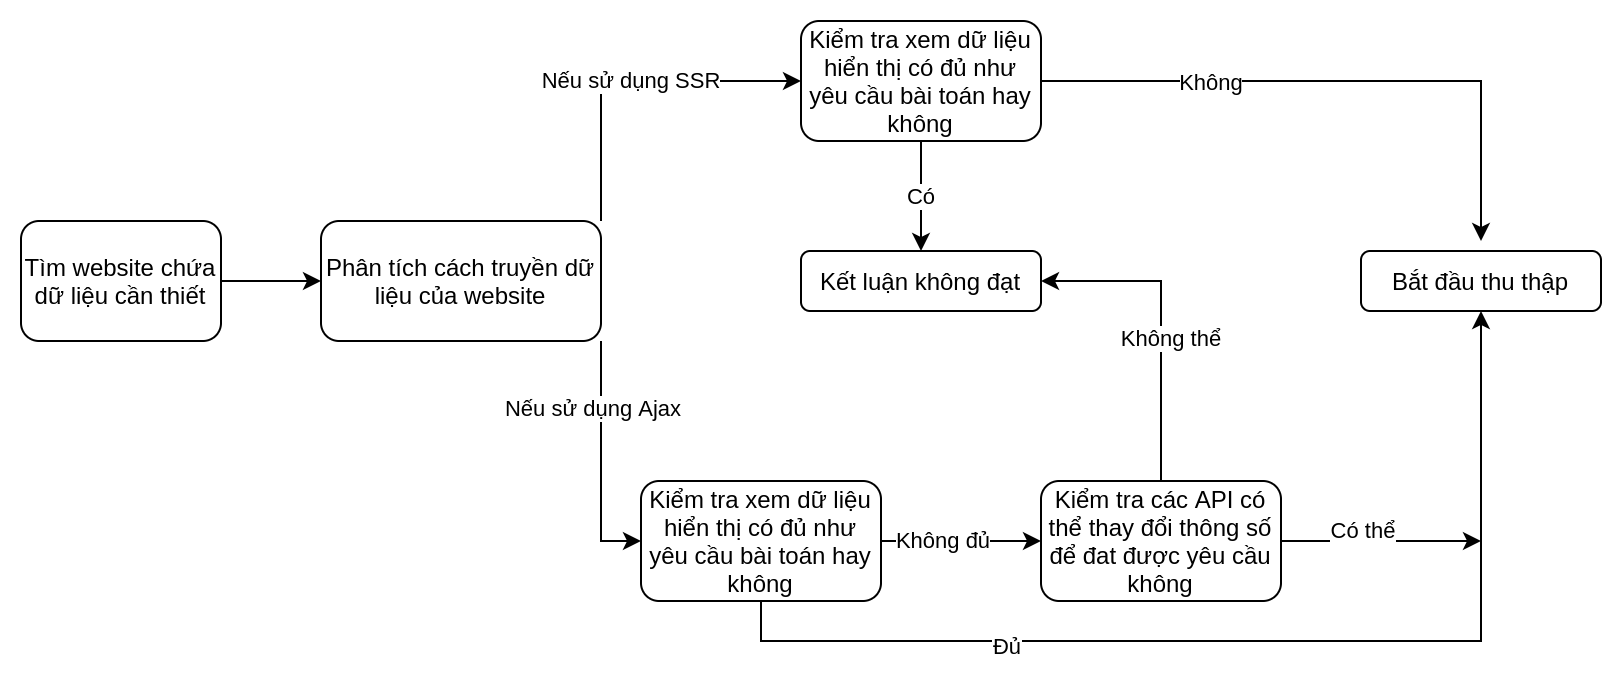
\includegraphics[width=6in]{images/process.png}

\subsubsection{weather.com}
\qquad Để tìm ra API phục vụ cho việc crawl ta vào trang Monthly của một địa phương cụ thể sau đó navigate đến các trang chứa dữ liệu của các tháng trước (việc này giúp cho website sử dụng các API yêu cầu dữ liệu thời tiết quá khứ). Kiểm tra các response trong filter XHR ta có thể tìm ra những response tốt nhất chứa dữ liệu cần thiết.

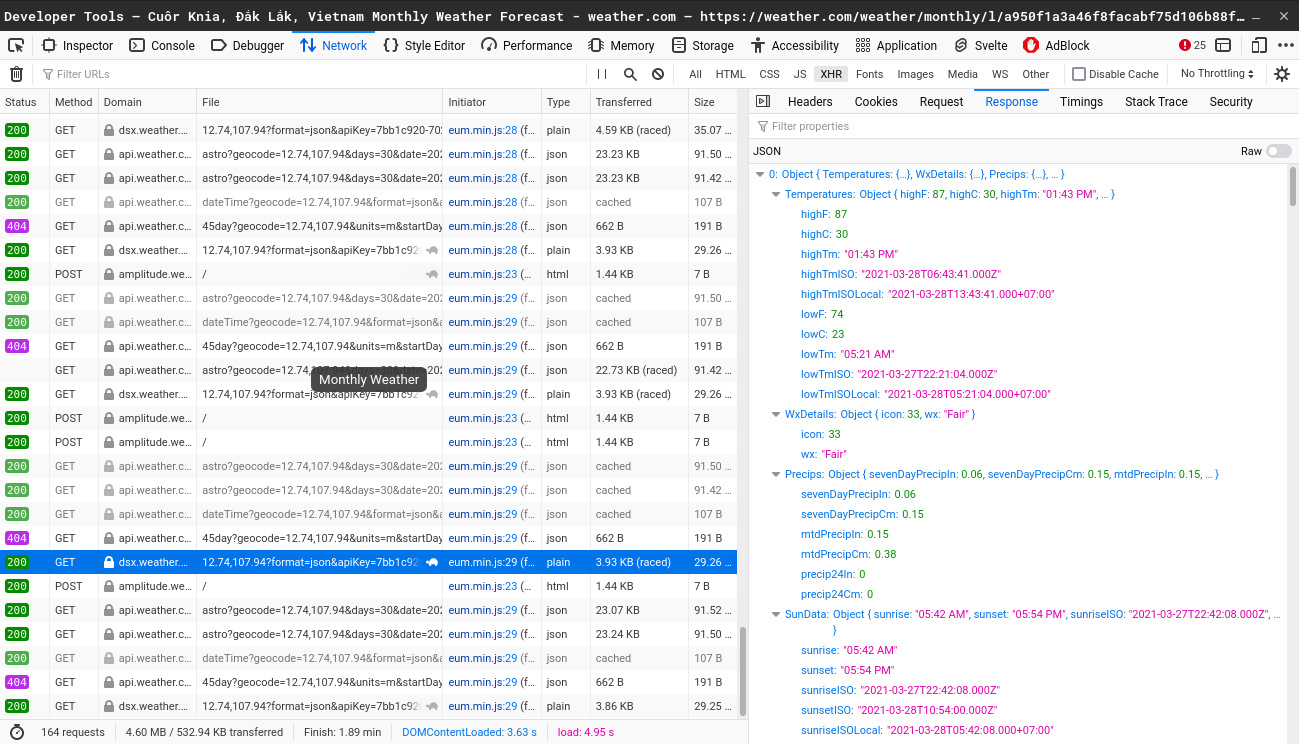
\includegraphics[width=6in]{images/inspect.png}

Tiếp theo đó khi đã xác nhận API này đủ điều kiện ra kiểm tra ý nghĩa của các thông số trong request, thử thay đổi thông số để kiểm tra dữ liệu kéo dài được đến bao lâu.

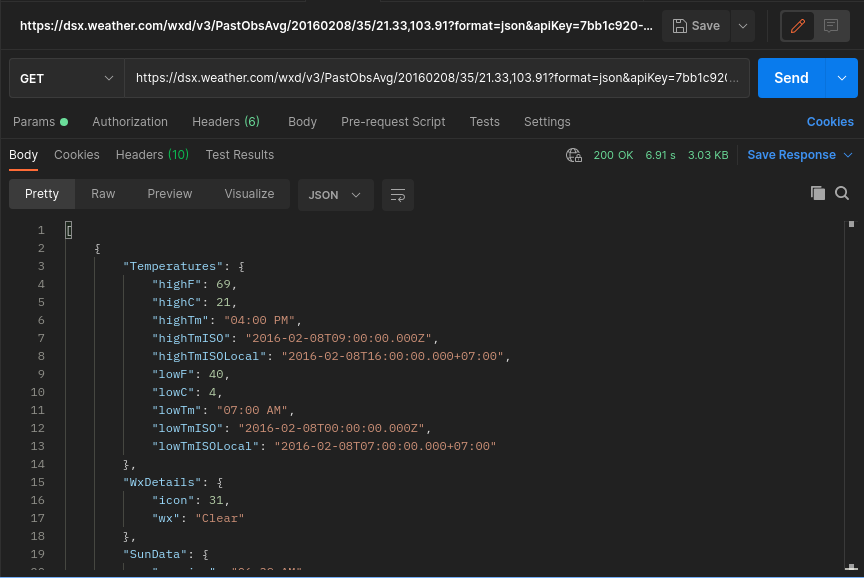
\includegraphics[width=6in]{images/checkpast.png}

Vì dữ liệu chấp nhận đến 2014 nên sẽ tiến hành crawl dữ liệu. Nhóm sử dụng Scrappy để crawl vì công cụ này hỗ trợ async cho phép gửi nhiều request cùng lúc cùng với đó là có pipeline để lưu dữ liệu nên giảm rất nhiều quá trình cài đặt.

% Continue here
Đầu tiên ta tạo tải dữ liệu danh sách chứa tất cả các xã cần crawl dữ liệu, làm tròn các tọa độ đến 2 chữ số thập phân(theo yêu cầu của API, xử lý bằng numpy trước sẽ nhanh hơn việc xử lý trong vòng lặp).

\begin{minted}[tabsize=4,breaklines]{python}
class IBMWeatherScapper(Spider):
    name = 'ibm-weather'

    df_ward_taynguyen_fire = pandas.read_csv(
        'https://raw.githubusercontent.com/.../taynguyen_wards_longlat.csv')
    df_ward_taynguyen_fire['long'] = numpy.round(
        df_ward_taynguyen_fire['long'], 2)
    df_ward_taynguyen_fire['lat'] = numpy.round(
        df_ward_taynguyen_fire['lat'], 2)
\end{minted}

Trong hàm start\_requests của Spider với mỗi xã ta tạo 1 request vào ngày 1/1/2014 với tọa độ của xã đó, cùng với đó là lưu kèm 1 meta để nhận diện xã đó trong parse function.

\begin{minted}[tabsize=4,breaklines]{python}
	def start_requests(self):
	requests = []
	for i, ward in self.df_ward_taynguyen_fire.iterrows():
		requests.append(request.Request(
			url=f"https://dsx.weather.com/wxd/v3/PastObsAvg/20140101/35/\
			{ward['lat']:.2f},{ward['long']:.2f}\
			?format=json\
			&apiKey=7bb1c920-7027-4289-9c96-ae5e263980bc&\
			fbclid=IwAR1IgpD8qPU6ZaHqDnZT1tMl95Y4G8gfGvIYmpM3CGGIqyjwQeaAmbZZ8SE",
			meta={
				'ward_code': ward['ward_code'],
				'long':ward['long'],
				'lat':ward['lat']
			},
			callback=self.parse
		))
	return requests
\end{minted}

Vì đây là API nên dữ liệu được thể hiện dưới dạng json rất rõ ràng.

\begin{minted}[tabsize=4,breaklines]{json}
	{
        "Temperatures": {
            "highF": 72,
            "highC": 22,
            "highTm": "01:00 PM",
            "highTmISO": "2014-01-01T06:00:00.000Z",
            "highTmISOLocal": "2014-01-01T13:00:00.000+07:00",
            "lowF": 68,
            "lowC": 20,
            "lowTm": "01:00 AM",
            "lowTmISO": "2013-12-31T18:00:00.000Z",
            "lowTmISOLocal": "2014-01-01T01:00:00.000+07:00"
        },
        "WxDetails": { "icon": 27, "wx": "Mostly Cloudy" },
        "SunData": {
            "sunrise": "06:05 AM",
            "sunset": "05:26 PM",
            "sunriseISO": "2013-12-31T23:05:00.000Z",
            "sunsetISO": "2014-01-01T10:26:00.000Z",
            "sunriseISOLocal": "2014-01-01T06:05:00.000+07:00",
            "sunsetISOLocal": "2014-01-01T17:26:00.000+07:00"
        },
        "Moon": {
            "moonriseLocal": "2014-01-01T05:34:00.000+07:00",
            "moonsetLocal": "2014-01-01T17:25:00.000+07:00",
            "moonriseISO": "2013-12-31T22:34:00.000Z",
            "moonsetlISO": "2014-01-01T10:25:00.000Z"
        }
    }
\end{minted}

Việc còn lại là lấy ra và lưu lại dưới file csv. Sau đó lấy ngày cuối cùng trong dữ liệu trả về xem có bằng ngày hôm nay không, nếu không thì tiếp tục tải dữ liệu còn nếu có thì dừng lại.

\begin{minted}[tabsize=4]{python}
	 def parse(self, response, **kwargs):
        json = response.json()
        ward_code = response.meta['ward_code']
        long = response.meta['long']
        lat = response.meta['lat']
        for d in json:
            yield {
                'ward':ward_code,
                'date':d.get('Temperatures', {}).get('highTmISOLocal','')[:10],
                'highC': d.get('Temperatures', {}).get('highC',''),
                'lowC': d.get('Temperatures', {}).get('lowC',''),
                'sun_rise': d.get('SunData', {}).get('sunrise',''),
                'sun_set': d.get('SunData',{}).get('sunset',''),
                'sevenDayPrecipCm':d.get('Precips',{}).get('sevenDayPrecipCm',''),
                'mtdPrecipCm':d.get('Precips',{}).get('mtdPrecipCm',''),
                'precip24Cm':d.get('Precips',{}).get('precip24Cm',''),
            }

		last = json[-1]
        recentDate = datetime.strptime(
            last['Temperatures']['highTmISO'][:10], '%Y-%M-%d')
        next = recentDate + timedelta(days=1)
		
		if recentDate.date() == datetime.today():
        	return
        else:
            yield response.follow(
                url=f"https://dsx.weather.com/wxd/v3/PastObsAvg/ \
				{next.strftime('%Y%M%d')}/35/{lat:.2f},{long:.2f}\
				?format=json\
				&apiKey=7bb1c920-7027-4289-9c96-ae5e263980bc\
				&fbclid=IwAR1IgpD8qPU6ZaHqDnZT1tMl95Y4G8gfGvIYmpM3CGGIqyjwQeaAmbZZ8SE",
                meta={
                        'ward_code': ward_code,
                        'long':long, 'lat':lat
                    },
                    callback=self.parse
            )
\end{minted}

Dữ liệu từ website này cung cấp có độ chính xác đến từng tọa độ, có nghĩa là chỉ cần cung cấp tọa độ (làm tròn đến 2 chữ số thập phân) thì server sẽ trả về thời tiết tại điểm đó tùy vào thời gian mà ta muốn. Tuy nhiên điểm yếu của dữ liệu này là chỉ cung cấp các đặc tính cơ bản nhất của thời tiết tại địa điểm đó gồm: nhiệt độ cao nhất và thấp nhất trong ngày, thời gian mặt trời mọc và lặn, lượng mưa (tích lũy trong 7 ngày, trong 1 tháng hoặc chỉ ngày hôm đó).

Sau khoảng nhiều ngày khai thác và xử lý, nhóm đã lấy được dữ liệu của 5 tỉnh Tây Nguyên vào từng xã từng ngày kéo dài từ 1/1/2014 đến 8/6/2021. Dữ liệu gồm các trường cơ bản sau (lưu ý các trường này đã được đổi tên so với khi crawl dữ liệu để thống nhất các bộ dữ liệu với nhau nhằm dễ dàng cho việc nghiên cứu):

\begin{itemize}
	\item ward: Mã của xã, phường, thị trấn, thị xã. Vì sẽ có những địa điểm trùng tên nên nhóm sử dụng mã để phân biệt các địa phương (mã này cung cấp bởi API của firewatchvn.kiemlam.org.vn\cite{website:firewatch_administrative})
	\item date: là ngày mà record được ghi lại.
	\item max/min: là nhiệt độ cao nhất và thấp nhất được ghi nhận trong ngày(celcius).
	\item sunrise/sunset: là thời gian mặt trời mọc và lặn.
	\item 7\_rain: lượng mưa tổng tính từ ngày chủ nhật gần nhất trước đó (cm)
	\item m\_rain: lượng mưa tổng tính từ ngày 1 của tháng đó(cm)
	\item 24\_rain: lượng mưa ghi nhận trong ngày(cm)
\end{itemize}

Dưới đây là một đoạn mẫu trong dữ liệu.

\begin{table}[H]
	\begin{tabular}{lllllllll}
		ward    & date       & max & min & sunrise  & sunset   & 7\_rain & m\_rain & 24\_rain \\
		24727.0 & 2016-10-17 & 30  & 25  & 05:36 AM & 05:28 PM & 5.94    & 30.91   & 1.82     \\
		24727.0 & 2016-10-18 & 30  & 25  & 05:36 AM & 05:28 PM & 7.54    & 32.66   & 1.75     \\
		24727.0 & 2016-10-19 & 30  & 25  & 05:36 AM & 05:27 PM & 7.54    & 32.96   & 0.3      \\
		24761.0 & 2019-10-14 & 32  & 24  & 05:36 AM & 05:30 PM & 0.02    & 0.07    & 0.0      \\
		24761.0 & 2019-10-15 & 32  & 25  & 05:36 AM & 05:30 PM & 0.02    & 0.07    & 0.0      \\
		24761.0 & 2019-10-16 & 32  & 25  & 05:36 AM & 05:29 PM & 0.02    & 0.07    & 0.02     \\
		24761.0 & 2019-10-17 & 32  & 25  & 05:36 AM & 05:29 PM & 0.02    & 0.07    & 0.0      \\
		24761.0 & 2019-10-18 & 32  & 25  & 05:36 AM & 05:28 PM & 0.02    & 0.07    & 0.0      \\
		24761.0 & 2019-10-19 & 32  & 26  & 05:36 AM & 05:28 PM & 0.02    & 0.07    & 0.0      \\
		24761.0 & 2019-10-20 & 32  & 26  & 05:36 AM & 05:27 PM & 0.02    & 0.1     & 0.0      \\
		24761.0 & 2019-10-21 & 33  & 25  & 05:36 AM & 05:27 PM & 0.02    & 0.1     & 0.0      \\
		24761.0 & 2019-10-22 & 32  & 25  & 05:37 AM & 05:26 PM & 0.02    & 0.1     & 0.0      \\
		24761.0 & 2019-10-23 & 33  & 25  & 05:37 AM & 05:26 PM & 0.0     & 0.1     & 0.0      \\
		24761.0 & 2019-10-24 & 33  & 25  & 05:37 AM & 05:25 PM & 0.0     & 0.1     & 0.0
	\end{tabular}
\end{table}

Dưới đây là các thông số của bộ dữ liệu

\begin{table}[H]
	\begin{tabular}{lllllll}
		      & ward    & max      & min      & 7\_rain   & m\_rain    & 24\_rain  \\
		count & 1130904 & 1130904  & 1130904  & 679514    & 679514     & 679514    \\
		mean  &         & 30.60013 & 24.66924 & 33.813765 & 82.088195  & 4.797731  \\
		std   &         & 2.836824 & 2.207649 & 71.482188 & 153.732438 & 16.574482 \\
		min   &         & 18       & 14       & 0         & 0          & 0         \\
		25\%  &         & 29       & 23       & 0.5       & 2.2        & 0         \\
		50\%  &         & 31       & 25       & 8.1       & 21.3       & 0         \\
		75\%  &         & 32       & 26       & 34.7      & 88.6       & 2.7       \\
		max   &         & 46       & 36       & 903.7     & 1300.7     & 419.1
	\end{tabular}
\end{table}

Kết quả trả về từ hàm nunique():

\begin{table}[H]
	\begin{tabular}{ll}
		ward     & 592  \\
		date     & 2739 \\
		max      & 25   \\
		min      & 21   \\
		sunrise  & 75   \\
		sunset   & 74   \\
		7\_rain  & 644  \\
		m\_rain  & 976  \\
		24\_rain & 231  \\
	\end{tabular}
\end{table}

Dữ liệu bị trống sau khi sắp xếp theo ngày và địa phương(theo thứ tự ngày trước địa phương sau, tăng dần):

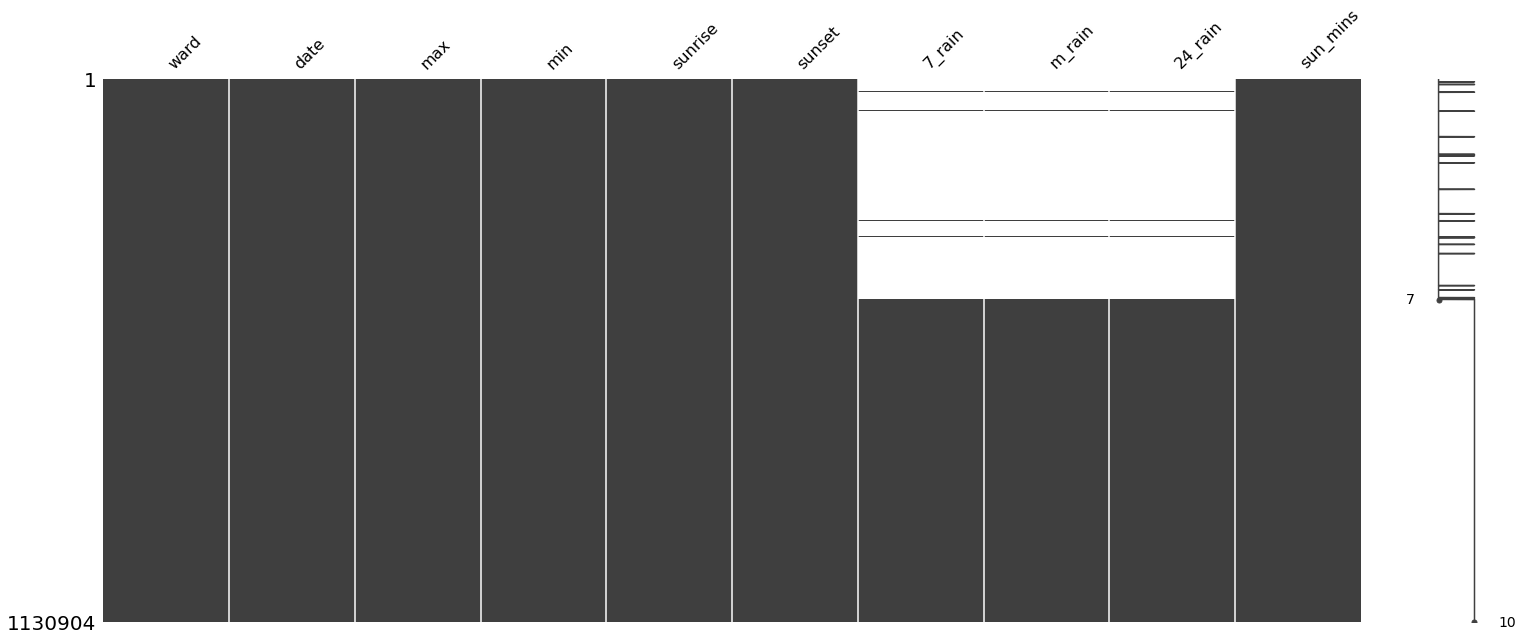
\includegraphics[width=6in]{images/missing.png}

\subsubsection{worldweatheronline.com}
\subsubsection{firewatchvn.kiemlam.org.vn}



\subsection{Xây dựng bộ dữ liệu}


\subsubsection{Imputation of Data}
\subsubsection{Creation of Dataset}


%----------------------------------------------------------------------------------------
%	SECTION 4
%----------------------------------------------------------------------------------------

\section{Training và đánh giá modelods}
% Chương này trình bày quá trình training và đánh giá các model mà nhóm đã thử. Đây là chương dài hơi và tốn thời gian nhất.
% Với mỗi model nhóm chọn thử nghiệm cần trình bày đầy đủ (1) nguồn tham khảo nếu như model đó tham khảo từ kết quả có trước. (2) Quá trình training thiết lập như thế nào, thời gian train, thời gian test, v.v..,

% Phần sau của chương trình bày kết quả đánh giá chi tiết model. Mỗi model phải show được các metric đánh giá performance.
% SHOW ĐƯỢC CÁC MẪU DỮ LIỆU mà model dự đoán sai và phân tích lý do. Đặc biệt chú ý các mẫu dữ liệu mà model này dự đoán đúng nhưng hầu hết model khác dự đoán sai, phải chụp ảnh được các mẫu dữ liệu đó làm ví dụ.
% Trình bày càng kỹ càng nhiều điểm

%----------------------------------------------------------------------------------------
%	SECTION 5

% Chương cuối trình bày khả năng ứng dụng của model, và hướng phát triển tiếp theo. Sẽ có điểm cộng nếu nhóm xây dựng được ứng dụng minh họa thực tế từ model đã train.

%----------------------------------------------------------------------------------------

\section{Ứng dụng và hướng phát triển}



%----------------------------------------------------------------------------------------
%	BIBLIOGRAPHY
%----------------------------------------------------------------------------------------

\bibliographystyle{plain}
\bibliography{source}

%----------------------------------------------------------------------------------------

\end{document}